\documentclass[11pt]{article}
\usepackage{etex}
\usepackage{amssymb,amsmath,fancyhdr,multicol}


\usepackage[metapost]{mfpic}

%\pgfplotsset{compat=1.9}
%\usepackage{amsmath}
\usepackage[pdftex]{graphicx}
%\usepackage{mystylefortest}
%\usepackage{multicol}
\usepackage{pst-plot}
\usepackage{pgfplots}

\usepackage{tikz}
\usepackage{tkz-2d}
\usepackage{tkz-base}
\usetikzlibrary{calc}

\usepackage[inline]{enumitem}

\textheight 25cm% 25.5cm
\textwidth 18cm \topmargin -2.5cm
\parindent 0pt
\oddsidemargin -1cm \columnsep 18pt 
\renewcommand{\headrulewidth}{0pt}
\pagestyle{fancy} \lhead{}\chead{}\rhead{}
\lfoot{}\cfoot{}\rfoot{}
%\newcommand{\ds}{\displaystyle}

\usepackage{tabularx}
\renewcommand{\tabularxcolumn}[1]{>{\centering\arraybackslash}m{#1}}

\usepackage{array}
\newcolumntype{?}{!{\vrule width 1pt}}

\usepackage[linewidth=1pt]{mdframed}

%\prec 
\pgfplotsset{compat=1.9} %%May have to change to 1.11 at work

\pgfplotsset{soldot/.style={color=blue,only marks,mark=*}} \pgfplotsset{holdot/.style={color=blue,fill=white,only marks,mark=*}}
\pgfplotsset{
  grid style = {
    dash pattern = on 0.05mm off 1mm,
    line cap = round,
    black,
    line width = 0.5pt
  }
}


\opengraphsfile{WorksheetExam1}

\begin{document}

\centerline{\textbf{Worksheet Exam 1}}

\vspace{.5in}

%\textbf{Name:}\hrulefill\

%\vspace{.25in}

%\makebox[\textwidth]{Name:\enspace\hrulefill}
%\vspace{1pt}

%\begin{questions}


%\addpoints
%\qformat{Question \thequestion\dotfill
 %        {(\pointsofquestion{\arabic{question}} \points)}}
        
\begin{enumerate}        
%%%%%%%%%%%%%%%%
\item The shaded region in the graph shown below represents a feasible region.

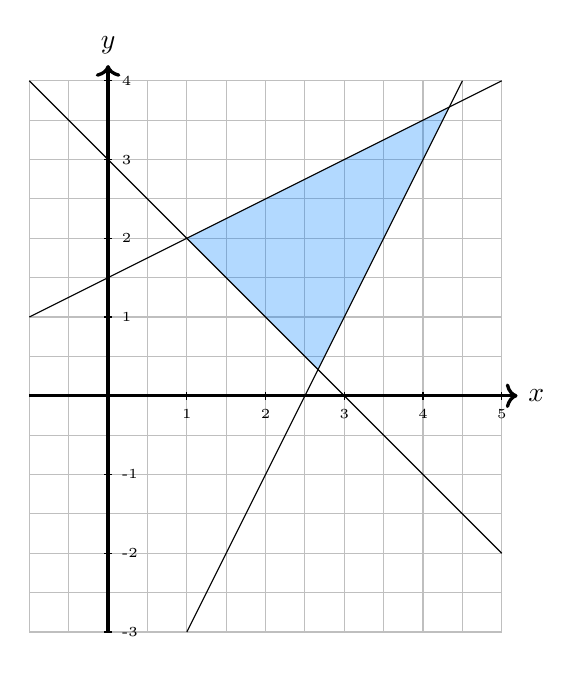
\begin{tikzpicture}

    \draw[gray!50, thin, step=0.5] (-1,-3) grid (5,4);
    \draw[very thick,->] (-1,0) -- (5.2,0) node[right] {$x$};
    \draw[very thick,->] (0,-3) -- (0,4.2) node[above] {$y$};

    \foreach \x in {1,...,5} \draw (\x,0.05) -- (\x,-0.05) node[below] {\tiny\x};
    \foreach \y in {1,...,4} \draw (-0.05,\y) -- (0.05,\y) node[right] {\tiny\y};
    \foreach \y in {-3,...,-1} \draw (-0.05,\y) -- (0.05,\y) node[right] {\tiny\y};

    \fill[blue!50!cyan,opacity=0.3] (8/3,1/3) -- (1,2) -- (13/3,11/3) -- cycle;

    \draw (-1,4) -- node[below,sloped] {} (5,-2);
    \draw (1,-3) -- (3,1) -- node[below left,sloped] {} (4.5,4);
    \draw (-1,1) -- node[above,sloped] {} (5,4);

\end{tikzpicture}



\begin{itemize} 
\item Is this statement true or false?  One of the inequalities which define the feasible region is $\displaystyle y\geq -x+3$. [Explain your reasoning.]
\item Is this statement true or false? If the objective function is $\displaystyle M=200-x-y$, then it is possible for the maximum of $M$ in the feasible region to be at $(2,2)$. [Explain your reasoning.]


\item Is this statement true or false? If the objective function is $\displaystyle M=200-x-y$, then it is possible for the maximum of $M$ in the feasible region to be at $(1,2)$.[Explain your reasoning.] 

\end{itemize}
\item (From Homework 1.) Consider the system of inequalities:

\[
\begin{cases}
    x>3\\
    y<5\\
    2x-4y>10 
\end{cases}
\]


\item (From Homework 1.) A trucker hauls citrus fruit from Florida to Montreal. Each crate of oranges is 4 ft${}^3$ in volume and weighs 80 lb. Each crate of grapefruit has a volume of 6 ft$\,^3$ and weighs 100 lb. His truck has a maximum capacity of 300 ft$\,^3$ and can carry no more than 6400 lb. Moreover, he is not permitted to carry more crates of grapefruit than crates of oranges. If his profit is \$2.50 on each crate of oranges and \$4 on each crate of grapefruit, how many crates of each fruit should he carry for maximum profit?

\item (From Homework 1.) A housing contractor has subdivided a farm into 100 building lots. She has designed two types of homes for these lots: colonial and ranch style. A colonial requires \$30,000 of capital and produces a profit of \$3000 when sold. A ranch-style house requires \$40,000 of capital and provides an \$9000 profit. If the contractor has \$3.6 million of capital on hand, how many houses of each type should she build for maximum profit?

\item (From Homework 1.) A woman wishes to invest \$11,500 in three types of bonds: municipal bonds paying 6\% interest per year, bank investment certificates paying 9\%, and high-risk bonds paying 13\%. For tax reasons she wants the amount invested in municipal bonds to be at least three times the amount invested in bank certificates. To keep her level of risk manageable, she will invest no more than \$1500 in high-risk bonds. How much should she invest in each type of bond to maximize her annual interest yield? [Hint: Let 
$x$ = amount in municipal bonds
 and 
$y$ = amount in bank certificates.
 Then the amount in high-risk bonds will be 
\$ $11,500 - x - y$.]

\item Does the relation $\displaystyle x+y^2=1$ represent a function? Explain your reasoning.

\item Sketch the graph of a function that has the specified domain and range.
\begin{itemize}
\item Domain $[0,1]$, range $[2,5]$
\item Domain $(0,1]$, range $(2,5]$
\item Domain $(-\infty,\infty)$, range $(-\infty,\infty)$
\item Domain $[0,\infty)$, range $[0.\infty)$
\item Domain $\{0,1,2,3\}$, range $\{4,5,6\}$
\item Domain $\displaystyle [-1.1]\cup [2,3]$, range $\displaystyle [0,1)\cup \{3\}$
\item Domain $\displaystyle (-1,0]\cup \{1,2\}$, range $\displaystyle  \{1,2,3\}$
\item Domain $(-\infty,\infty)$, range $\displaystyle \{ 1\}$
\item Domain $[0,\infty)$, range $(-\infty,\infty)$
\item Domain $[0,1)$, range $[0.\infty)$
\item Domain $\displaystyle [0, 1) \cup (1, 2]$, range $(-\infty,\infty)$
\end{itemize}

\item What number must be in the range of a function $f$ if the graph of $f$ has an $x$-intercept?
Explain your answer.

\item What number must be in the domain of a function $f$ if the graph of $f$ has a $y$-intercept?
Explain your answer.

\item Why is it impossible to have a function like $\displaystyle f(x)=\sqrt{x-2} + \sqrt{1-x}$? 

\item Sketch the graph of a function with  all of these characteristics:
\begin{itemize}
\item The points $(-10, 5)$ and $(0,-5)$ are local maximums on the graph of $y = f (x)$
\item The points $(1, 0)$ and $(2, 0)$ are x-intercepts of the graph of $y = f (x)$
\end{itemize}



\item Determine if the relation whose graph is below represents $y$ as a function of $x$.  If so, state the domain and range using interval notation.

\begin{enumerate}
\begin{multicols}{2}

\item $~$ \vspace{-.1in}

\begin{mfpic}[17]{-5}{2}{-2}{5}
\circle{(-3,2.5),2}
\axes
\tlabel[cc](2,-0.5){\scriptsize $x$}
\tlabel[cc](0.5,4.75){\scriptsize $y$}
\xmarks{-4,-3,-2,-1,1}
\ymarks{-1,1,2,3,4}
\tlpointsep{4pt}
\axislabels {x}{{\tiny $-4 \hspace{6pt}$} -4, {\tiny $-3 \hspace{6pt}$} -3, {\tiny $-2 \hspace{6pt}$} -2, {\tiny $-1 \hspace{6pt}$} -1, {\tiny $1$} 1}
\axislabels {y}{{\tiny $-1$} -1, {\tiny $1$} 1, {\tiny $2$} 2, {\tiny $3$} 3, {\tiny $4$} 4}
\end{mfpic}

\item $~$

\begin{mfpic}[17]{-4.5}{5.5}{-4}{3}

\arrow \polyline{(-1,2),(-4,3)}
\arrow \function{1,4,0.1}{1-(x-2)**2}
\gclear \circle{(-1,2),0.1}
\circle{(-1,2),0.1}
\gfill \circle{(1,0),0.1}


\axes
\tlabel[cc](5.5,-0.5){\scriptsize $x$}
\tlabel[cc](0.5,2.75){\scriptsize $y$}
\xmarks{-4,-3,-2,-1,1,2,3,4,5}
\ymarks{-3,-2,-1,1,2}
\tlpointsep{4pt}
\axislabels {x}{{\tiny $-4 \hspace{6pt}$} -4, {\tiny $-3 \hspace{6pt}$} -3, {\tiny $-2 \hspace{6pt}$} -2, {\tiny $-1 \hspace{6pt}$} -1, {\tiny $1$} 1, {\tiny $2$} 2, {\tiny $3$} 3, {\tiny $4$} 4, {\tiny $5$} 5}
\axislabels {y}{{\tiny $-3$} -3, {\tiny $-2$} -2, {\tiny $-1$} -1, {\tiny $1$} 1, {\tiny $2$} 2}
\end{mfpic}

\end{multicols}

\end{enumerate}




%%%%%%%%%%%%%%%%%%%%%%
%\begin{enumerate}

\item  Suppose $f$ is a function that takes a real number $x$ and performs the following steps in the order given:  

\smallskip

(1) add 4

\smallskip

(2) take the square root

\smallskip

(3) subtract 5 

\smallskip

(4) divide into 10

\smallskip

Find an expression for $f(x)$ and state the domain of $f$ using interval notation.

%\vspace{.25in}

\item Find the domain of the function $\displaystyle f(x)=\sqrt{x^2+2x-3}$ and write it in interval form.

\item Find the domain of the function $\displaystyle f(x)=\frac{1}{x^2+2x-3}$ and write it in interval form.


\item  Let $f(x) = \left\{ \begin{array}{rr}  3x - 1, & x \leq -4 \\ -x^2, & x > -4 \\  \end{array}\right.$.  Find $f(-2)$, $f(-4)$,  and $f(-5)$.

%\end{enumerate}




\item  Given the graph of $y = f(x)$ below, answer all of the following questions.
\label{tame}

\begin{center}

\begin{mfpic}[20]{-5}{5}{-5}{5}
\point[3pt]{(-2,0), (2,0), (4,-3), (-4,-3), (0,3)}
\function{-4,4,.1}{3*cos(3.14159265*x/4)}
\tlabel[cc](-3,0.5){\small $\left( -2, 0 \right)$}
\tlabel[cc](2.5,0.5){\small $\left(2, 0 \right)$}
\tlabel[cc](4,-3.5){\small $\left( 4, -3 \right)$}
\tlabel[cc](-4,-3.5){\small $\left(-4, -3 \right)$}
\tlabel[cc](1,3.5){\small $\left(0, 3 \right)$}
\axes
\tlabel[cc](5,-0.5){\scriptsize $x$}
\tlabel[cc](0.5,5){\scriptsize $y$}
\xmarks{-4,-3,-2,-1,1,2,3,4}
\ymarks{-4,-3,-2,-1,1,2,3,4}
\tlpointsep{5pt}
\scriptsize
\axislabels {x}{{$-4 \hspace{7pt}$} -4, {$-3 \hspace{7pt}$} -3, {$-2 \hspace{7pt}$} -2, {$-1 \hspace{7pt}$} -1, {$1$} 1, {$2$} 2, {$3$} 3, {$4$} 4}
\axislabels {y}{{$-4$} -4, {$-3$} -3, {$-2$} -2, {$-1$} -1, {$1$} 1, {$2$} 2, {$3$} 3, {$4$} 4}
\normalsize
\end{mfpic}

\end{center}

\begin{multicols}{2}
\begin{enumerate}

\item  Find the domain of $f$.

\item  Find the range of $f$.

%\setcounter{enumi}{\value{HW}}

\item  List the $x$-intercepts, if any exist.

\item  List the $y$-intercepts, if any exist.


%\setcounter{enumi}{\value{HW}}

\item  Find the zeros of $f$.

\item  Solve $f(x) < 0$.


%\setcounter{enumi}{\value{HW}}

\item  Determine $f(2)$.

\item  Solve $f(x) = -3$.  


%\setcounter{enumi}{\value{HW}}

\item  Find the number of solutions to $f(x) = 1$.

\item  Does $f$ appear to be even, odd, or neither?


%\setcounter{enumi}{\value{HW}}

\item  List the intervals on which $f$ is increasing.

\item  List the intervals on which $f$ is decreasing.


%\setcounter{enumi}{\value{HW}}

\item  List the local maximums, if any exist.

\item  List the local minimums, if any exist.


%\setcounter{enumi}{\value{HW}}

\item  Find the maximum, if it exists.

\item  Find the minimum, if it exists.

%\setcounter{HW}{\value{enumi}}
\end{enumerate}
\end{multicols}


\item Use the graph of $y = f(x)$ given below to answer the  questions listed below.

\begin{center}

\begin{mfpic}[15]{-5}{5}{-6}{6}
\function{-4, 4, 0.1}{5*sin(x*3.14159/4)}
\point[3pt]{ (-2, -5), (0, 0), (4,0), (2,3), (-4,0)}
\pointfillfalse
\point[3pt]{(2,5)}
\axes
\tlabel[cc](5,-0.5){\scriptsize $x$}
\tlabel[cc](0.5,6){\scriptsize $y$}
\xmarks{-3,-2,-1,1,2,3,4}
\ymarks{-5,-4,-3,-2,-1,1,2,3,4,5}
\tlpointsep{5pt}
\scriptsize
\axislabels {x}{{$-4 \hspace{7pt}$} -4, {$-3 \hspace{7pt}$} -3,{$-2 \hspace{7pt}$} -2, {$-1 \hspace{7pt}$} -1, {$1$} 1, {$2$} 2, {$3$} 3, {$4$} 4}
\axislabels {y}{{$-5$} -5,{$-4$} -4,{$-3$} -3,{$-2$} -2,{$-1$} -1, {$1$} 1, {$2$} 2, {$3$} 3, {$4$} 4, {$5$} 5}
\normalsize
\end{mfpic}

\end{center}

\begin{multicols}{2}
\begin{enumerate}


\item  Find the domain of $f$. \label{usesecondfuncgraphfirst}
\item  Find the range of $f$.



\item  Determine $f(2)$.
\item  Solve $f(x) = -5$.



\item  List the $x$-intercepts, if any exist.
\item  List the $y$-intercepts, if any exist.



\item  Find the zeros of $f$.
\item  Solve $f(x) \leq 0$.



\item  Find the number of solutions to $f(x) = 3$.
\item  Does $f$ appear to be even, odd, or neither?



\item  List the intervals where $f$ is increasing.
\item  List the intervals where $f$ is decreasing.



\item  List the local maximums, if any exist.
\item  List the local minimums, if any exist.



\item  Find the maximum, if it exists.
\item  Find the minimum, if it exists. \label{usesecondfuncgraphlast}


\end{enumerate}
\end{multicols}

\item The complete graph of $y=f(x)$ is given below.

\begin{center}

\begin{mfpic}[15]{-1}{6}{-1}{6}

\polyline{(0,1), (2,3), (4,2), (5,0)}

\point[3pt]{(0,1), (2,3), (4,2), (5,0)}

\tlabel[cc](-1,1){\scriptsize $(0,1)$}

\tlabel[cc](2,3.5){\scriptsize $(2,3)$}

\tlabel[cc](4.5,2.5){\scriptsize $(4,2)$}

\tlabel[cc](5,-0.5){\scriptsize $(5,0)$}

\tlabel[cc](6,-0.5){\scriptsize $x$}

\tlabel[cc](0.5,6){\scriptsize $y$}


\tcaption{\scriptsize $y=f(x)$}

\axes

\xmarks{1,2,3,4,5}

\ymarks{1,2,3,4,5}

\tlpointsep{4pt}

\axislabels {x}{{\tiny $1$} 1, {\tiny $2$} 2, {\tiny $3$} 3, {\tiny $4$} 4}

\axislabels {y}{{\tiny $2$} 2, {\tiny $3$} 3, {\tiny $4$} 4, {\tiny $5$} 5}

\end{mfpic}

\end{center}

\begin{multicols}{2}
\begin{enumerate}
\item Write the domain in interval form.
\item Write the range in interval form.
\item What are the global maxima, if they exist?
\item What are the global minima, if they exist?
\item Fill each of the tables. If a value is undefined, write NONE.
\begin{enumerate}
\item 
\begin{tabular}{|l|l|l|l|l|l|l|l|l|}
\hline
$x$    & -1 & 0 & 1 & 2 & 3 & 4 & 5 & 6 \\ \hline
$f(x)$ &    &   &   &   &   &   &   &   \\ \hline
\end{tabular}
%\end{table}
\item 

%\begin{table}[h]
\begin{tabular}{|l|l|l|l|l|l|l|l|l|}
\hline
$x$    & -1 & 0 & 1 & 2 & 3 & 4 & 5 & 6 \\ \hline
$f(x+1)$ &    &   &   &   &   &   &   &   \\ \hline
\end{tabular}
\item 

%\begin{table}[h]
\begin{tabular}{|l|l|l|l|l|l|l|l|l|}
\hline
$x$    & -1 & 0 & 1 & 2 & 3 & 4 & 5 & 6 \\ \hline
$f(x-1)$ &    &   &   &   &   &   &   &   \\ \hline
\end{tabular}
\item 

%\begin{table}[h]
\begin{tabular}{|l|l|l|l|l|l|l|l|l|}
\hline
$x$    & -1 & 0 & 1 & 2 & 3 & 4 & 5 & 6 \\ \hline
$2f(x)$ &    &   &   &   &   &   &   &   \\ \hline
\end{tabular}
\item 

%\begin{table}[h]
\begin{tabular}{|l|l|l|l|l|l|l|l|l|}
\hline
$x$    & -1 & 0 & 1 & 2 & 3 & 4 & 5 & 6 \\ \hline
$f(2x)$ &    &   &   &   &   &   &   &   \\ \hline
\end{tabular}
\item 

%\begin{table}[h]
\begin{tabular}{|l|l|l|l|l|l|l|l|l|}
\hline
$x$    & -1 & 0 & 1 & 2 & 3 & 4 & 5 & 6 \\ \hline
$\displaystyle \frac{f(x)}{2}$ &    &   &   &   &   &   &   &   \\ \hline
\end{tabular}
\item 

%\begin{table}[h]
\begin{tabular}{|l|l|l|l|l|l|l|l|l|}
\hline
$x$    & -1 & 0 & 1 & 2 & 3 & 4 & 5 & 6 \\ \hline
$\displaystyle f\left (\frac{x}{2}\right )$ &    &   &   &   &   &   &   &   \\ \hline
\end{tabular}
\end{enumerate}

\end{enumerate}
\end{multicols}


\item The graph of two functions $f(x)$ and $g(x)$ are shown below. What is the formula for $g(x)$?

\begin{minipage}[t]{0.5\linewidth}
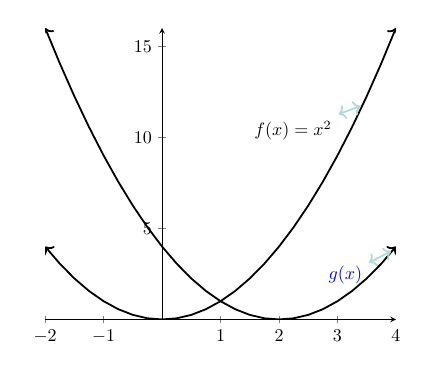
\begin{tikzpicture}[scale=0.65]
\begin{axis}[
    domain=-2:4,
    axis y line=center,
        axis x line=middle,
]
%\addplot [no markers,line width=1pt,<->] {x^2} node [pos=0.3,left] {$f(x)=x^2$};
\addplot [no markers,line width=1pt,<->]{x^2}
    %node[pos=0.1,pin=135:{\color{purple}$f(x)=-2$}] {}
    node [pos=0.8,pin={200:$f(x)=x^2$},inner sep=0pt] {};
    %node[pos=0.9,pin=135:{\color{green!70!black}$f(x)=3$}] {}
;
\addplot [no markers,line width=1pt,<->]{(x-2)^2}
    %node[pos=0.1,pin=135:{\color{purple}$f(x)=-2$}] {}
    node[pos=0.99,pin=200:{\color{blue}$g(x)$},inner sep=0pt] {}
    %node[pos=0.9,pin=135:{\color{green!70!black}$f(x)=3$}] {}
;
\end{axis}
\end{tikzpicture}
\end{minipage}%
\begin{minipage}[b]{0.5\linewidth}
\begin{enumerate}
\item $g(x)=x^2+2$
\item $g(x)=x^2-2$
\item $g(x)=(x+2)^2$
\item $g(x)=(x-2)^2$
\end{enumerate}
\end{minipage}


\item The graph of a function $f(x)$ is shown below.






\pgfmathdeclarefunction{f}{1}{%
        \pgfmathparse{#1*#1*(-0.5)+2*#1+1}%
    }
    % or \pgfmathdeclarefunction{f}{1}{\pgfmathparse{#1*#1}}

        \fbox{\begin{tikzpicture}[baseline=(current bounding box.north),scale=0.5]
            \begin{axis}[
        axis y line=center,
        axis x line=middle, 
         xmin=0,
        xmax=4,
        ymin=0,
        ymax=4,
        xlabel=\scalebox{1.5}{$x$},
        ylabel=$y$,
        x label style={at={(current axis.right of origin)},anchor=north, below=5mm},
        y label style={at={(current axis.above origin)},rotate=0,anchor=south east,left=5mm},
         clip=false,
				grid=both,
				minor xtick={0,1,...,4},
				minor ytick={1,2,...,4},
        enlarge x limits=0,
        scaled x ticks = true
      ]
                \addplot[domain=0:4,blue,line width=2.0pt] {f(x)}; %no shift (clearly centered
                %\addplot {f(x-1)}; %little shift to the right
                %\addplot {f(2*x)}; %shifted nearly off the sheet
                \draw [draw=blue, fill=blue, thick] (axis cs: 0, 1) circle (5.0pt);
                \draw [draw=blue, fill=blue, thick] (axis cs: 4, 1) circle (5.0pt);
            \end{axis}
            \node[below, yshift=-4mm] at (current bounding box.south) {Function $f(x)$};
       \end{tikzpicture}
}     
\parbox[t]{11cm}{\vskip0pt
   Match each graph with one of the transformations of $f$ from the list
of possible answers given below. Write the transformation on the dotted line below each graph.


\begin{mdframed}[leftmargin=10pt,rightmargin=10pt]
%{\renewcommand{\arraystretch}{2}%
\begin{tabular*}{0.95\textwidth}{ccccc}
%\hline
\multicolumn{5}{c}{\textbf{Possible Answers}}\\
%\hline
$f(x)+1$ & $f(x+1)$& $f(-x)$ & $f(2x)$& $-f(x)$ \\
$\displaystyle f\left (\frac{x}{2}\right )$ & $\displaystyle \frac{1}{2}f(x)$ &$f(x)-1$ & $f(x-1)$ & $2f(x)$ \\ 
\end{tabular*}
\end{mdframed}
}

%%%%%%%%%%%%%%

\pgfplotsset{
    standard/.style={
        axis x line=middle,
        axis y line=middle,
        enlarge x limits=0.15,
        enlarge y limits=0.15,
        every axis x label/.style={at={(current axis.right of origin)},anchor=north west},
        every axis y label/.style={at={(current axis.above origin)},anchor=north east}
    }
}

\begin{figure}[h]
\hspace*{\fill}
\begin{tikzpicture}[scale=0.5]
            \begin{axis}[
        axis y line=center,
        axis x line=middle, 
         xmin=0,
        xmax=5,
        ymin=0,
        ymax=4,
        xlabel=\scalebox{1.5}{$x$},
        ylabel=\scalebox{1.5}{$y$},
        %x label style={at={(current axis.right of origin)},anchor=north, below=5mm},
        %y label style={at={(current axis.above origin)},rotate=0,anchor=south east,left=5mm},
         clip=false,
				grid=both,
				minor xtick={0,1,...,4},
				minor ytick={1,2,...,4},
        enlarge x limits=0,
        scaled x ticks = true
      ]
                \addplot[domain=1:5,blue,line width=2.0pt] {f(x-1)}; %no shift (clearly centered
                %\addplot {f(x-1)}; %little shift to the right
                %\addplot {f(2*x)}; %shifted nearly off the sheet
                \draw [draw=blue, fill=blue, thick] (axis cs: 1, 1) circle (5.0pt);
                \draw [draw=blue, fill=blue, thick] (axis cs: 5, 1) circle (5.0pt);
            \end{axis}
       %\end{tikzpicture} 
\node[below, yshift=-4mm] at (current bounding box.south) {\hbox to 1in{\dotfill}};
\end{tikzpicture}\hspace*{\fill}
\begin{tikzpicture}[scale=0.5]
            \begin{axis}[
        axis y line=center,
        axis x line=middle, 
         xmin=-1,
        xmax=4,
        ymin=0,
        ymax=4,
        xlabel=\scalebox{1.5}{$x$},
        ylabel=\scalebox{1.5}{$y$},
        %axis labels at tip,
        %x label style={at={(current axis.right of origin)},anchor=north, below=5mm},
        %y label style={at={(current axis.above origin)},rotate=0,anchor=north,left=5mm,yshift=1.5ex},
         clip=false,
				grid=both,
				minor xtick={0,1,...,4},
				minor ytick={1,2,...,4},
        enlarge x limits=0,
        scaled x ticks = true
      ]
                \addplot[domain=-1:3,blue,line width=2.0pt] {f(x+1)}; %no shift (clearly centered
                %\addplot {f(x-1)}; %little shift to the right
                %\addplot {f(2*x)}; %shifted nearly off the sheet
                \draw [draw=blue, fill=blue, thick] (axis cs: -1, 1) circle (5.0pt);
                \draw [draw=blue, fill=blue, thick] (axis cs: 3, 1) circle (5.0pt);
            \end{axis}
       %\end{tikzpicture} 
\node[below, yshift=-4mm] at (current bounding box.south) {\hbox to 1in{\dotfill}};
\end{tikzpicture}\hspace*{\fill}
\begin{tikzpicture}[scale=0.5]
            \begin{axis}[
        axis y line=center,
        axis x line=middle, 
         xmin=-4,
        xmax=0,
        ymin=0,
        ymax=4,
        xlabel=\scalebox{1.5}{$x$},
        ylabel=\scalebox{1.5}{$y$},
        %axis labels at tip,
        %x label style={at={(current axis.right of origin)},anchor=north, below=5mm},
        %y label style={at={(current axis.above origin)},rotate=0,anchor=north,left=5mm,yshift=1.5ex},
         clip=false,
				grid=both,
				minor xtick={-4,-3,...,-1},
				minor ytick={1,2,...,4},
        enlarge x limits=0,
        scaled x ticks = true
      ]
                \addplot[domain=-4:0,blue,line width=2.0pt] {f(-x)}; %no shift (clearly centered
                %\addplot {f(x-1)}; %little shift to the right
                %\addplot {f(2*x)}; %shifted nearly off the sheet
                \draw [draw=blue, fill=blue, thick] (axis cs: -4, 1) circle (5.0pt);
                \draw [draw=blue, fill=blue, thick] (axis cs: 0, 1) circle (5.0pt);
            \end{axis}
       %\end{tikzpicture} 
\node[below, yshift=-4mm] at (current bounding box.south) {\hbox to 1in{\dotfill}};
\end{tikzpicture}\hspace*{\fill}
%\caption{Two figures side by-side}
%\label{fig:test}
\end{figure}
%%%%%%%%%%%%%%%%%%%%
\begin{figure}[h]
\hspace*{\fill}
\begin{tikzpicture}[scale=0.5]
            \begin{axis}[
        axis y line=center,
        axis x line=middle, 
         xmin=0,
        xmax=4,
        ymin=0,
        ymax=2,
        xlabel=\scalebox{1.5}{$x$},
        ylabel=\scalebox{1.5}{$y$},
        %x label style={at={(current axis.right of origin)},anchor=north, below=5mm},
        %y label style={at={(current axis.above origin)},rotate=0,anchor=south east,left=5mm},
         clip=false,
				grid=both,
				minor xtick={1,2,3,4},
				minor ytick={1,2},
				enlarge x limits=0,
        scaled x ticks = true
      ]
                \addplot[domain=0:4,blue,line width=2.0pt] {0.5*f(x)}; %no shift (clearly centered
                %\addplot {f(x-1)}; %little shift to the right
                %\addplot {f(2*x)}; %shifted nearly off the sheet
                \draw [draw=blue, fill=blue, thick] (axis cs: 0, 0.5) circle (5.0pt);
                \draw [draw=blue, fill=blue, thick] (axis cs: 4, 0.5) circle (5.0pt);
            \end{axis}
       %\end{tikzpicture} 
\node[below, yshift=-4mm] at (current bounding box.south) {\hbox to 1in{\dotfill}};
\end{tikzpicture}\hspace*{\fill}
\begin{tikzpicture}[scale=0.5]
            \begin{axis}[
        axis y line=center,
        axis x line=middle, 
         xmin=0,
        xmax=4,
        ymin=0,
        ymax=6,
        xlabel=\scalebox{1.5}{$x$},
        ylabel=\scalebox{1.5}{$y$},
        %axis labels at tip,
        %x label style={at={(current axis.right of origin)},anchor=north, below=5mm},
        %y label style={at={(current axis.above origin)},rotate=0,anchor=north,left=5mm,yshift=1.5ex},
         clip=false,
				grid=both,
				minor xtick={0,1,...,4},
				minor ytick={1,2,...,6},
        enlarge x limits=0,
        scaled x ticks = true
      ]
                \addplot[domain=0:4,blue,line width=2.0pt] {2*f(x)}; %no shift (clearly centered
                %\addplot {f(x-1)}; %little shift to the right
                %\addplot {f(2*x)}; %shifted nearly off the sheet
                \draw [draw=blue, fill=blue, thick] (axis cs: 0, 2) circle (5.0pt);
                \draw [draw=blue, fill=blue, thick] (axis cs: 4, 2) circle (5.0pt);
            \end{axis}
       %\end{tikzpicture} 
\node[below, yshift=-4mm] at (current bounding box.south) {\hbox to 1in{\dotfill}};
\end{tikzpicture}\hspace*{\fill}
\begin{tikzpicture}[scale=0.5]
            \begin{axis}[
        axis y line=center,
        axis x line=middle, 
         xmin=0,
        xmax=2,
        ymin=0,
        ymax=4,
        xlabel=\scalebox{1.5}{$x$},
        ylabel=\scalebox{1.5}{$y$},
        %axis labels at tip,
        %x label style={at={(current axis.right of origin)},anchor=north, below=5mm},
        %y label style={at={(current axis.above origin)},rotate=0,anchor=north,left=5mm,yshift=1.5ex},
         clip=false,
				grid=both,
				minor xtick={0,1,2},
				minor ytick={1,2,...,4},
        enlarge x limits=0,
        scaled x ticks = true
      ]
                \addplot[domain=0:2,blue,line width=2.0pt] {f(2*x)}; %no shift (clearly centered
                %\addplot {f(x-1)}; %little shift to the right
                %\addplot {f(2*x)}; %shifted nearly off the sheet
                \draw [draw=blue, fill=blue, thick] (axis cs: 0, 1) circle (5.0pt);
                \draw [draw=blue, fill=blue, thick] (axis cs: 2, 1) circle (5.0pt);
            \end{axis}
       %\end{tikzpicture} 
\node[below, yshift=-4mm] at (current bounding box.south) {\hbox to 1in{\dotfill}};
\end{tikzpicture}\hspace*{\fill}
%\caption{Two figures side by-side}
%\label{fig:test}
\end{figure}
%%%%%%%%%%%%%%%%%%%%
\begin{figure}[h]
\hspace*{\fill}
\begin{tikzpicture}[scale=0.5]
            \begin{axis}[
        axis y line=center,
        axis x line=middle, 
         xmin=0,
        xmax=4,
        ymin=-3,
        ymax=1,
        xlabel=\scalebox{1.5}{$x$},
        ylabel=\scalebox{1.5}{$y$},
        %x label style={at={(current axis.right of origin)},anchor=north, below=5mm},
        %y label style={at={(current axis.above origin)},rotate=0,anchor=south east,left=5mm},
         clip=false,
				grid=both,
				minor xtick={1,2,3,4},
				minor ytick={-3,-2,-1,1},
				enlarge x limits=0,
        scaled x ticks = true
      ]
                \addplot[domain=0:4,blue,line width=2.0pt] {-f(x)}; %no shift (clearly centered
                %\addplot {f(x-1)}; %little shift to the right
                %\addplot {f(2*x)}; %shifted nearly off the sheet
                \draw [draw=blue, fill=blue, thick] (axis cs: 0, -1) circle (5.0pt);
                \draw [draw=blue, fill=blue, thick] (axis cs: 4, -1) circle (5.0pt);
            \end{axis}
       %\end{tikzpicture} 
\node[below, yshift=-4mm] at (current bounding box.south) {\hbox to 1in{\dotfill}};
\end{tikzpicture}\hspace*{\fill}
\begin{tikzpicture}[scale=0.5]
            \begin{axis}[
        axis y line=center,
        axis x line=middle, 
         xmin=0,
        xmax=8,
        ymin=0,
        ymax=3,
        xlabel=\scalebox{1.5}{$x$},
        ylabel=\scalebox{1.5}{$y$},
        %axis labels at tip,
        %x label style={at={(current axis.right of origin)},anchor=north, below=5mm},
        %y label style={at={(current axis.above origin)},rotate=0,anchor=north,left=5mm,yshift=1.5ex},
         clip=false,
				grid=both,
				minor xtick={0,2,...,8},
				minor ytick={1,2,3},
        enlarge x limits=0,
        scaled x ticks = true
      ]
                \addplot[domain=0:8,blue,line width=2.0pt] {f(0.5*x)}; %no shift (clearly centered
                %\addplot {f(x-1)}; %little shift to the right
                %\addplot {f(2*x)}; %shifted nearly off the sheet
                \draw [draw=blue, fill=blue, thick] (axis cs: 0, 1) circle (5.0pt);
                \draw [draw=blue, fill=blue, thick] (axis cs: 8, 1) circle (5.0pt);
            \end{axis}
       %\end{tikzpicture} 
\node[below, yshift=-4mm] at (current bounding box.south) {\hbox to 1in{\dotfill}};
\end{tikzpicture}\hspace*{\fill}
\begin{tikzpicture}[scale=0.5]
            \begin{axis}[
        axis y line=center,
        axis x line=middle, 
         xmin=0,
        xmax=4,
        ymin=0,
        ymax=3,
        xlabel=\scalebox{1.5}{$x$},
        ylabel=\scalebox{1.5}{$y$},
        %axis labels at tip,
        %x label style={at={(current axis.right of origin)},anchor=north, below=5mm},
        %y label style={at={(current axis.above origin)},rotate=0,anchor=north,left=5mm,yshift=1.5ex},
         clip=false,
				grid=both,
				minor xtick={0,1,2,3,4},
				minor ytick={1,2,3},
        enlarge x limits=0,
        scaled x ticks = true
      ]
                \addplot[domain=0:4,blue,line width=2.0pt] {f(x)-1}; %no shift (clearly centered
                %\addplot {f(x-1)}; %little shift to the right
                %\addplot {f(2*x)}; %shifted nearly off the sheet
                \draw [draw=blue, fill=blue, thick] (axis cs: 0, 0) circle (5.0pt);
                \draw [draw=blue, fill=blue, thick] (axis cs: 4, 0) circle (5.0pt);
            \end{axis}
       %\end{tikzpicture} 
\node[below, yshift=-4mm] at (current bounding box.south) {\hbox to 1in{\dotfill}};
\end{tikzpicture}\hspace*{\fill}
%\caption{Two figures side by-side}
%\label{fig:test}
\end{figure}

%%%%%%%%%%%%%%%%%
\item The range of a function $y=f(x)$ is $[0,4]$. Then the range of the function transformation $2f\left( x\right)$ is 
\begin{enumerate}
\item $[0,4]$;
\item $[0,8]$;
\item $[0,2]$;
\item
 $[0,1]$.
\end{enumerate}

\item  Suppose you have a function $y= f(x)$ such that the domain of $f(x)$ is $1 \leq  x \leq  6$ and
the range of $f(x)$ is $-3 \leq  y \leq  5$. 
\begin{enumerate}
\item What is the domain of $f(2(x-3))$?
\item What is the range of $f(2(x-3))$?
\item What is the domain of $2f(x)-3$?
\item What is the range of $2f(x)-3$?
\item Can you find constants B and C so that the domain of $f(B(x-C))$  is $8 \leq  x \leq 9$?
\item Can you find constants A and D so that the range of $Af(x)+D$ is $0 \leq  y \leq  1$?
\end{enumerate}


%%%%%%%%%%^^^^^
\item Find the domain and range of the function shown below. (Enter your answers using interval notation.) 

\begin{mfpic}[15]{-4}{4}{-5}{5}
\point[3pt]{(-2,0),  (1,-2), (3,0)}
 \function{-2,1,0.1}{4-x**2}
\function{1,3,0.1}{x-3}
\gclear \circle{(1,3),0.1}
\gclear \circle{(0,4),0.1}
\gclear \circle{(1,-2),0.1}
\circle{(1,3),0.1}
\circle{(0,4),0.1}
\circle{(1,-2),0.1}
\axes
\tlabel[cc](4,-0.5){$x$}
\tlabel[cc](0.5,5){$y$}
\xmarks{-3,-2,-1,1,2,3}
\ymarks{-4,-3,-2,-1,1,2,3,4}
\tlpointsep{5pt}
\scriptsize
\axislabels {x}{{$-3 \hspace{7pt}$} -3, {$-2 \hspace{7pt}$} -2, {$-1 \hspace{7pt}$} -1, {$1$} 1, {$2$} 2, {$3$} 3}
\axislabels {y}{{$-4$} -4,{$-3$} -3,{$-2$} -2,{$-1$} -1, {$1$} 1, {$2$} 2, {$3$} 3, {$4$} 4}
\normalsize
\end{mfpic}

\item The graph of a function is given:

\includegraphics[width=2.5cm]{maxmin1.png}

\begin{enumerate}
\item (From Homework 2) Find all the local maximum and minimum values of the function as well as the value of $x$ at which each occurs. 

\begin{enumerate}
\item local maximum	$(x, y) =\,\,$ (smaller x-value)
\item local maximum	$(x, y) =\,\,$ (larger x-value)
\item local minimum	$(x, y) =\,\,$ (smaller x-value)
\item local minimum	$(x, y) =\,\,$ (larger x-value)
\end{enumerate}
\item  Find the intervals on which the function is increasing, and on which the function is decreasing. (Enter your answers using interval notation.) 
\end{enumerate}


\item (From Homework 2) Find the domain of the function $\displaystyle g(x) = x^2 - 3x - 18$. (Enter your answer using interval notation.)

\item Is the line $y=3$ a one-to-one function?

\item Is the line $x=3$ a one-to-one function?

\item   The domain of a function $y=f(x)$ is $[0,4]$. Then the domain of the function transformation $f\left( \frac{1}{2}x\right)$ is 
\begin{enumerate*}[series=MyList, before=\hspace{-0.6ex}]
\item $[0,4]$;
\item  $[0,8]$;
\item  $[0,2]$;
\item  $[0,1]$.
\end{enumerate*}

\item   The domain of a function $y=f(x)$ is $[0,4]$. Then the domain of the function transformation $f(2x)$ is 
\begin{enumerate*}[series=MyList, before=\hspace{-0.6ex}]
\item $[0,4]$;
\item  $[0,8]$;
\item  $[0,2]$;
\item  $[0,1]$.
\end{enumerate*}

\item  The range of a function $y=f(x)$ is $[0,4]$. Then the range of the function transformation $f\left( \frac{1}{2}x\right)$ is 
\begin{enumerate*}[series=MyList, before=\hspace{-0.6ex}]
\item $[0,4]$;
\item  $[0,8]$;
\item  $[0,2]$;
\item  $[0,1]$.
\end{enumerate*}

\item  The graph shown below on the left represents a function $f(x)$. Then the graph shown below on the right represents the function $f(2x+2)$. 
\begin{enumerate*}[series=MyList, before=\hspace{-0.6ex}]
\item True
\item False
\end{enumerate*}


\begin{minipage}[c]{0.40\linewidth}
				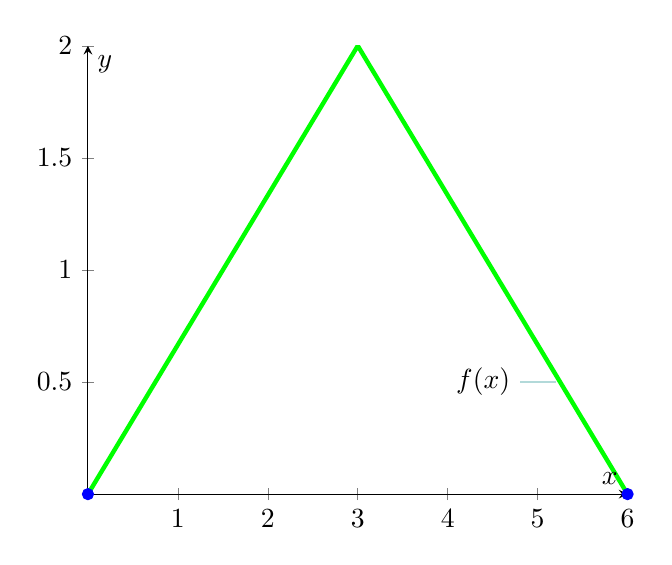
\begin{tikzpicture}
\begin{axis}[axis y line=center,
	axis x line=middle,xlabel=$x$,ylabel=$y$]
  \addplot[ultra thick,green]
  coordinates 
	{(0,0) (3,2) (6,0)};
	\node[coordinate,pin=left:{$f(x)$}]
at (axis cs:5.2,0.5) {};
\addplot[soldot] coordinates{(0,0)(6,0)};	
\end{axis}
\end{tikzpicture}
\end{minipage}
\hfill  \hfill
\begin{minipage}[c]{0.40\linewidth}
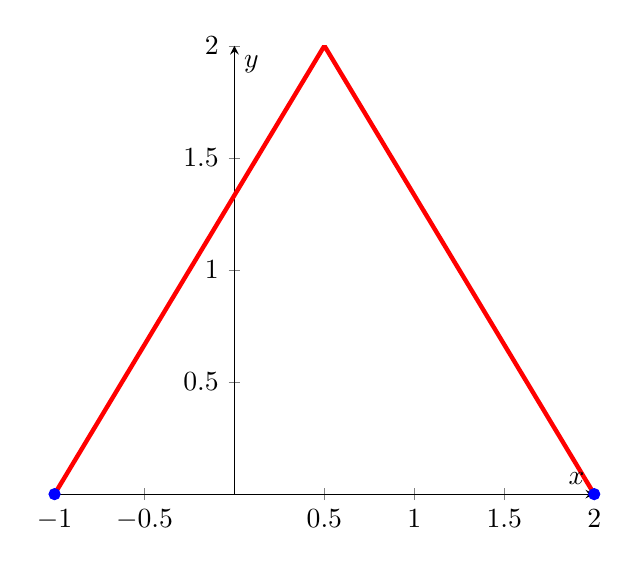
\begin{tikzpicture}
\begin{axis}[axis y line=center,
	axis x line=middle,xlabel=$x$,ylabel=$y$]

 \addplot[ultra thick,red]
  coordinates 
	{(-1,0) (0.5,2) (2,0)};
\addplot[soldot] coordinates{(-1,0)(2,0)};	  
\end{axis}
\end{tikzpicture}
\end{minipage}

\item Write a formula for the function obtained from $\displaystyle y=\sqrt{x}$ by applying the following transformations (in the given order): 
\begin{enumerate*}[series=MyList, before=\hspace{-0.6ex}] 
\item reflection around the $y$ axis; \item horizontal shift by 3 units to the left.
\end{enumerate*}

\item Write a formula for the function obtained from $\displaystyle y=\sqrt{x}$ by applying the following transformations (in the given order): 
\begin{enumerate*}[series=MyList, before=\hspace{-0.6ex}] 
 \item horizontal shift by 3 units to the right;
\item reflection around the $y$ axis.
\end{enumerate*}

\item Write a formula for the function obtained from $\displaystyle y=\sqrt{x}$ by applying the following transformations (in the given order): 
\begin{enumerate*}[series=MyList, before=\hspace{-0.6ex}] 
\item reflection around the $y$ axis; \item horizontal shift by 3 units to the right.
\end{enumerate*}

\item Write a formula for the function obtained from $\displaystyle y=\sqrt{x}$ by applying the following transformations (in the given order): 
\begin{enumerate*}[series=MyList, before=\hspace{-0.6ex}] 
 \item horizontal shift by 3 units to the left;
\item reflection around the $y$ axis.
\end{enumerate*}

\item The graph of a function $h(x)$ is shown below. Find all values of $x$ for which $h(x)\geq 3$ and write your answer in interval form. Explain how you arrived at your answer. 

\begin{center}
\begin{tikzpicture}[scale=0.6]
\tkzInit[xmin=0,xmax=10,xstep=1,ymin=0,ymax=7,ystep=1]
\tkzGrid[sub,subxstep=5,subystep=250,%
color=blue,subcolor=blue!50]%
\tkzX[orig,label = x]
\tkzY[orig,label = y]
\tkzSetOfPoints(%
0/2,%
2/4,%
4/3,%
10/7)
\tkzSegment[lw=2pt](tkzPt1/tkzPt2,tkzPt2/tkzPt3,tkzPt3/tkzPt4)
\SetUpPoint[mark=*,size=4pt,color=black]
\tkzPoint[name=$ $](0,2){A}
\tkzPoint[name=$ $](10,7){B}
\end{tikzpicture}
\end{center}

\item A tank holds 100 gallons of water, which drains from a leak at the bottom, causing the tank to empty in 40 minutes. Torricelli's Law gives the volume of water remaining in the tank after $t$ minutes as $\displaystyle V(t)=100\left (1-\frac{t}{40}\right )^2$.

\begin{enumerate}
\item What does $V(20)$ represent in practical terms? Does the number 20 represent a time or a volume?
\item What does $\displaystyle V^{-1}(20)$ represent in practical terms? Does the number 20 represent a time or a volume?
\end{enumerate}

\item (From Homework 3) A function $f$ is given, and the indicated transformations are applied to its graph (in the given order). Write the equation for the final transformed graph:
$\displaystyle f(x) = |x|$;
 shrink vertically by a factor of $\displaystyle \frac{1}{6}$, 
shift to the left 6 units, and shift upward 9 units.

\item (From Homework 3) Let 
$\displaystyle f(x) = x^2$.
 Find a formula for a function $g$ whose graph is obtained from the graph of 
$y = f(x)$ after the following sequence of transformations (in the given order):
\begin{enumerate*}[series=MyList, before=\hspace{-0.6ex}] 
\item  Shift left 4 units.
\item Reflection across the $y$-axis.
\item Shift down 3 units.
\item Vertical scaling by a factor of 3.
\item Reflection across the $x$-axis.
\end{enumerate*}


%%%%%%%%%%^^^^^^


\end{enumerate}
\end{document}